\chapter{MapReduce} % (fold)
\label{cha:background}

%This chapter introduces some concepts that are used in the subsequent sections: the MapReduce programming model and its constituents,
%and the bacteriological algorithm, used to generate and evolve test data. 

%\section{MapReduce}\label{section:mapreduce}
MapReduce~\cite{dean:2008} is a programming model and a paradigm to build
large-scale parallel data processing applications. The programming model is inspired
on the \textit{Map} and \textit{Reduce} primitives from functional programming
languages. The framework proposes two extensions points (or hooks), whose interface
is based on this same two higher-order functions. Users create MapReduce programs
(or jobs) by defining the precise behavior of these functions.

During execution, the framework deploys copies of the program across several
worker nodes, partitions the input data and schedules the execution across a set
of nodes. The framework also handles node failures and the required communication
between nodes. After the deployment, the master selects idle workers to assign a
map or a reduce instance and orchestrates their execution. The data flow between
the map and the reduce functions is shown in Figure~\ref{fig:mrexecute}.

\begin{figure}[htbp]
	\centering
	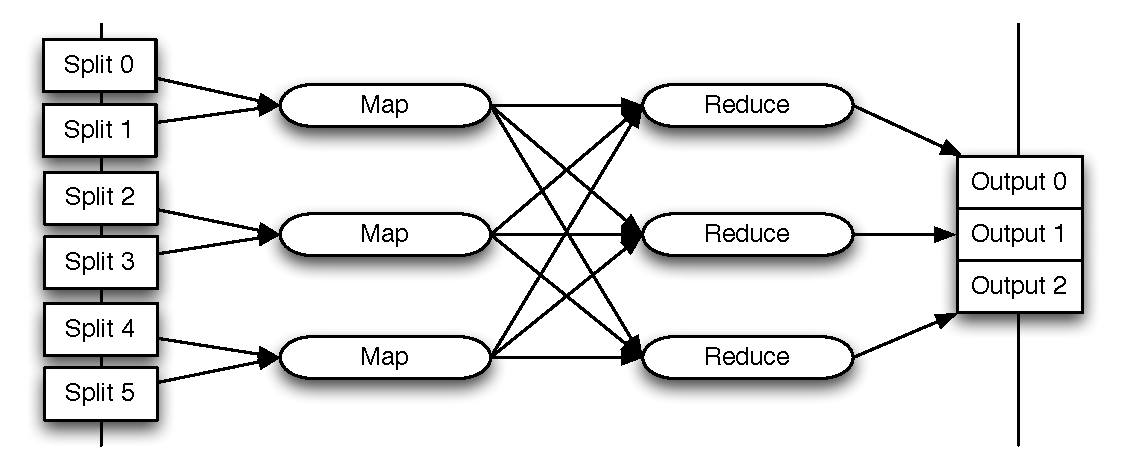
\includegraphics[width=\columnwidth]{img/mapreduce-en.pdf}
%    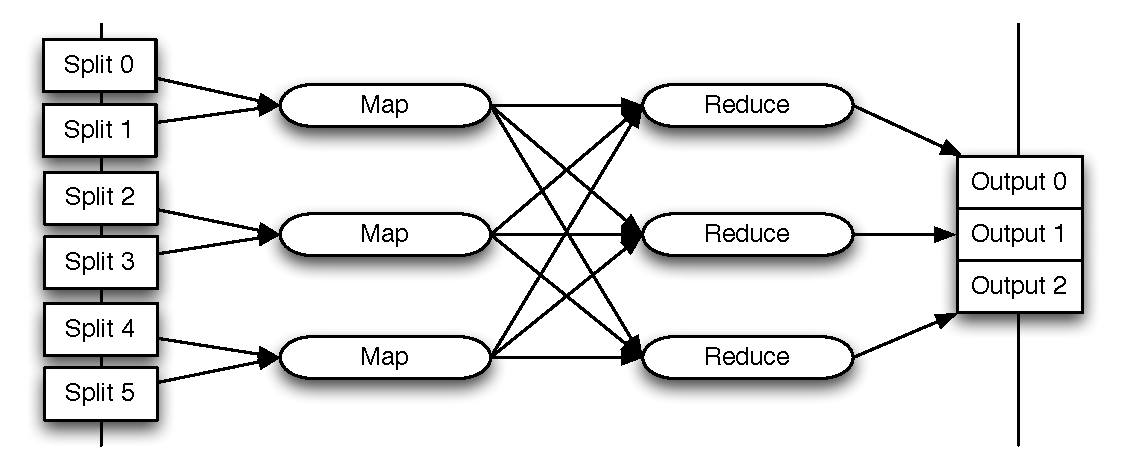
\includegraphics[bb=0 0 1280 960]{img/mapreduce-en.pdf}
	\caption{Execution of Map and Reduce operations}\label{fig:mrexecute}
\end{figure}

The input data set is divided into several \emph{splits}. 
Each split is assigned to a map task and executed on a node. 
The result of this processing is a set of intermediate keys and associated values. 
Reduce tasks take the results from map tasks to produce the final result.
When all the reduce instances terminate, they append their result to the final output file.

The whole processing is based on \tuple{key,value} pairs. 
The Map function groups together all input values $v1$ associated to the
same key $k1$ into an intermediate result set of keys and values \tuple{k2,v2}. 
These values are passed to the Reduce function that combines them into a reduced set: 

\begin{center}
\begin{tabular}{c c c c}
	\hline
	   map & $k1,v1$ & $\rightarrow$  & $set(k2, v2)$ \\
	   reduce & $k2, set(v2)$ & $\rightarrow$ & $set(v2)$ \\
	\hline
\end{tabular}
\end{center}

Eventually, the data flow may be completed with a \emph{Combiner}, a local reduce function used for bandwidth optimization.
This function runs after the Mapper and before the Reducer and is run on every node that has run map functions.
The Combiner may be seen as a \emph{mini-reduce} function, which operates only on data generated by one machine.

A canonical example of a MapReduce job is the Word Count application, which has as an input several textual documents and as an output a set of pairs \tuple{Key,Value}, where each key is a different word and the value is the number of occurrences of the word on all input documents.
The responsibility of  of the Mapper is to separate the text into a set of words and that of the Reducer is to aggregate matchings words and count the number of occurrences.
In this example, the function of the Combiner is almost identical to that of the Reducer. The main difference is that combiners are executed locally to each node, immediately after each mapper, and use local data, while reducers execute on different nodes and use data that comes from different mappers.

The Java implementation of the map function is presented in Listing~\ref{listing:mapper}. 
The \code{map()} method has three parameters: \code{key}, which is never used; \code{value}, which contains the text to be processed; and \code{context}, which will receive the output pairs.
The body of the method uses the class \code{StringTokenizer} to break the input text into tokens and then, for each token, writes a pair containing the token and the number 1.
The map does not count words, if there are several occurrences of a word in the input, there will also be several occurrences of it in the output.

\singlespacing
\begin{listing}[H]
\begin{minted}[frame=lines,framesep=2mm,fontfamily=courier,fontsize=\scriptsize]{java}
public static class TokenizerMapper extends Mapper<Object, Text, Text, IntWritable> {
   
    private final static IntWritable one = new IntWritable(1);
    private Text word = new Text();
   
    @Override
    public void map(Object key, Text value, Context context) 
                   throws IOException, InterruptedException {

        StringTokenizer itr = new StringTokenizer(value.toString());
      
        while (itr.hasMoreTokens()) {
            word.set(itr.nextToken());
            context.write(word, one);
        }
    }
}
\end{minted}
\caption{Class TokenizerMapper} 
\label{listing:mapper}
\end{listing}

\doublespacing
The implementation of the reduce function is presented in Listing~\ref{listing:reducer}.
The \code{reduce()} method has also three parameters: \code{key}, which contains a single word; \code{values}, a set containing all values associated to the key (i.e. the word); and \code{context}, the output.
The behavior of the method is quite simple, it sums all values associated to the key and then writes a pair containing the same key and the calculated amount.
\singlespacing
\begin{listing}[H]
\begin{minted}[frame=lines,framesep=2mm,fontfamily=courier,fontsize=\scriptsize]{java}
public static class IntSumReducer extends Reducer<Text, IntWritable, Text, IntWritable> {

    private IntWritable result = new IntWritable();

    @Override
    public void reduce(Text key, Iterable<IntWritable> values, Context context)
                      throws IOException, InterruptedException {
	
        int sum = 0;
        for (IntWritable val : values) {
            sum += val.get();
        }
        result.set(sum);
        context.write(key, result);
    }
}
\end{minted}
\caption{Class IntSumReducer} 
\label{listing:reducer}
\end{listing}

\doublespacing
Eventually, the reduce function could also be used as a combiner, to locally aggregate different occurrences of the same word.
The choice of using or not a combiner, as well as the number of reducer instances, is not automatic, it is left to developer.
Still, this choice may have an important impact in both, the correctness and the efficiency of the job.
An example of the inputs and the outputs of both functions when applied to a simple sentence is presented in Table~\ref{table:wordcount}.


\begin{table}[H]
	\begin{center}
	\begin{tabular}{c p{.4\columnwidth} c p{.3\columnwidth} }
		\hline
		map & "Never Say Never Again" & $\rightarrow$ & \tuple{Never,1},\tuple{Say,1}, \tuple{Never,1}, \tuple{Again,1} \\
		reduce & \tuple{Never,\{1,1\}}, \tuple{Say,\{1\}}, \tuple{Again,\{1\}} & $\rightarrow$ & \tuple{Never,2},\tuple{Say,1}, \tuple{Again,1}\\
		\hline
	\end{tabular}
	\end{center}
	\caption{Word count example}
	\label{table:wordcount}
\end{table}

% chapter chapter_name (end)
